\documentclass[12pt, a4paper]{article}

\usepackage[utf8]{inputenc}
\usepackage[T1]{fontenc}
\usepackage[francais]{babel}
\usepackage[top=1.5cm, bottom=1.2cm, left=1.2cm, right=2cm]{geometry}
\usepackage{verbatim}
\usepackage{graphicx}
\usepackage{listings}
\usepackage[dvipsnames]{xcolor}

\lstset{
%upquote=true,
columns=flexible,
basicstyle=\ttfamily,}

\title{Projet IHM -- Rapport 3 -- RICM4}
\author{\bsc{Fréby} Rodolphe -- \bsc{Barbier} Jérome -- \bsc{Husson} Augustin -- \bsc{Labat} Paul}
\date{\today}


\begin{document}
\maketitle
\tableofcontents
\newpage

\textcolor{Violet}{\section{Introduction}}
Voici le 3ème et dernier rapport du projet d'IHM. Il a pour objectif de présenter les critères de Scapin et Bastien que notre prototype respecte, après une description de ces fonctionnalités.

\textcolor{Violet}{\section{Organisation de la fenêtre}}

Tout d'abord, la hiérarchie des objets de l'interface est la suivante :

\begin{figure}[h]
\begin{center}
   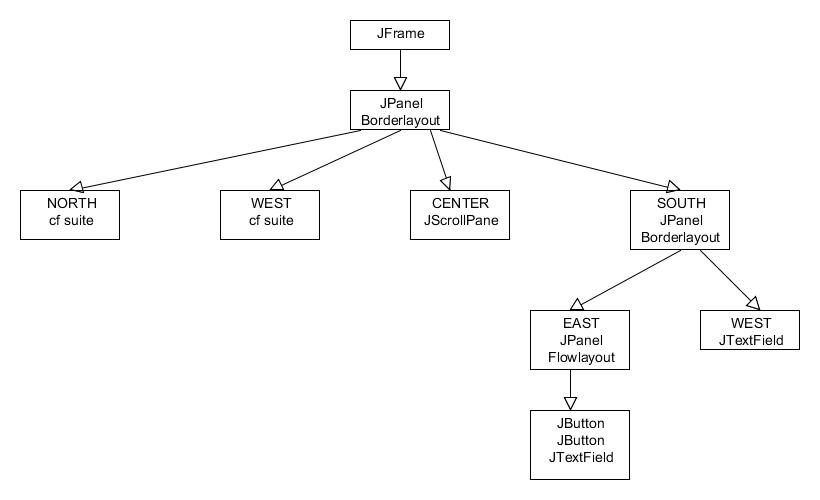
\includegraphics[scale = 0.65]{arbre_jframe.jpg}
	\caption{Hiérarchie des objets de notre interface}
	\end{center}
\end{figure}

La totalité du dessin étant trop gros pour être laissé sur une seule image, voici les éléments \emph{NORTH} et \emph{WEST} non présent sur le schéma ci-dessus. Les accolades signales un sous menu dans un JMenu, pour éviter de surcharger le dessin en faisant de nouvelles cases, ce qui reviendrait à un dessin beaucoup trop large.
\newpage
\begin{figure}[!h]
\begin{center}
   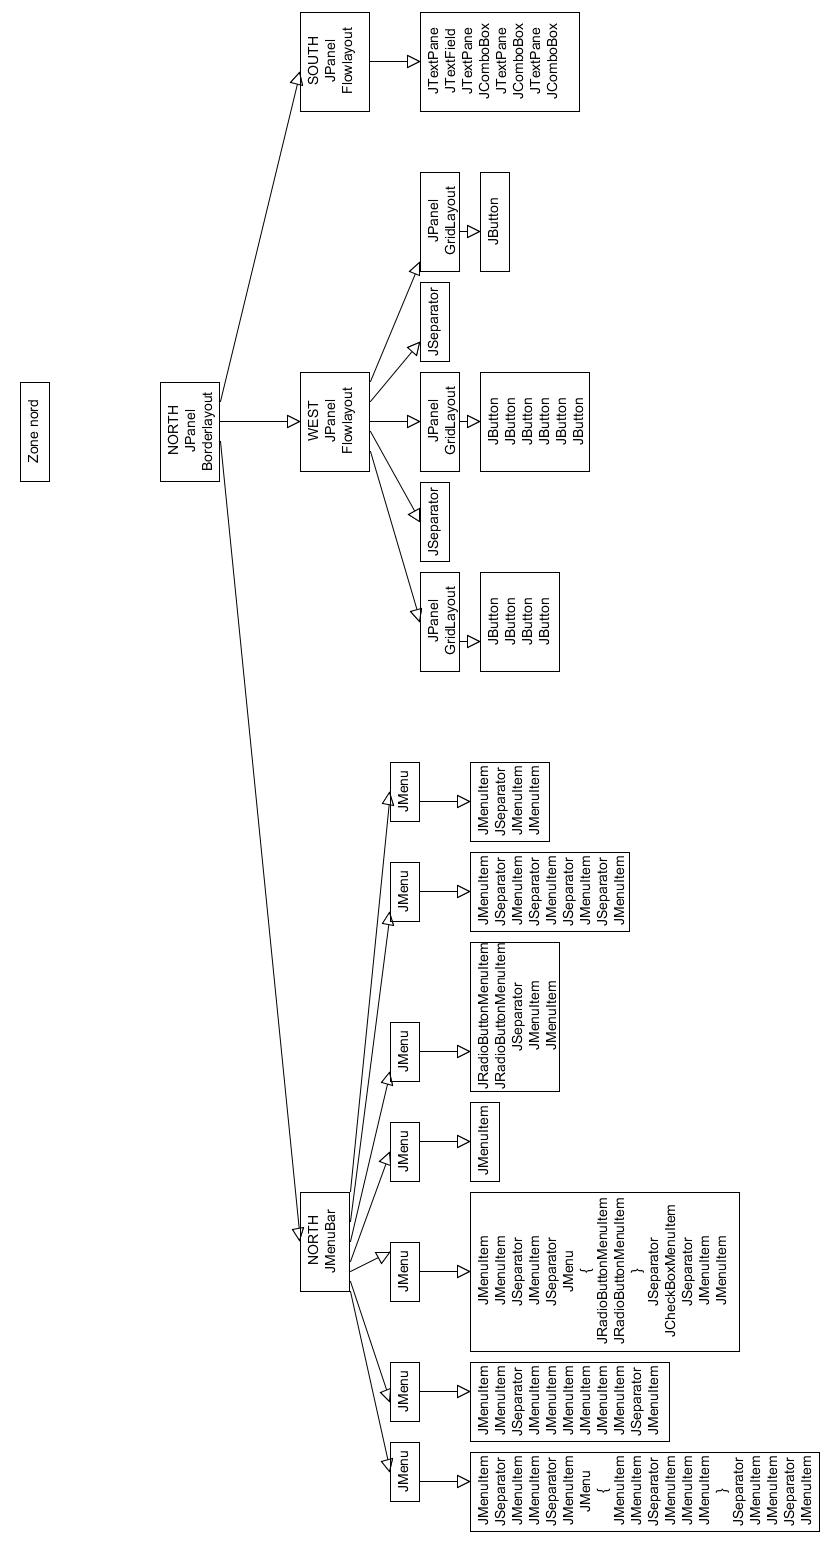
\includegraphics[scale = 0.43]{arbre_jframe_nord.jpg}
	\caption{Hiérarchie des objets de la zone nord de la fenêtre}
	\end{center}
\end{figure}
\newpage
\begin{figure}[!h]
\begin{center}
   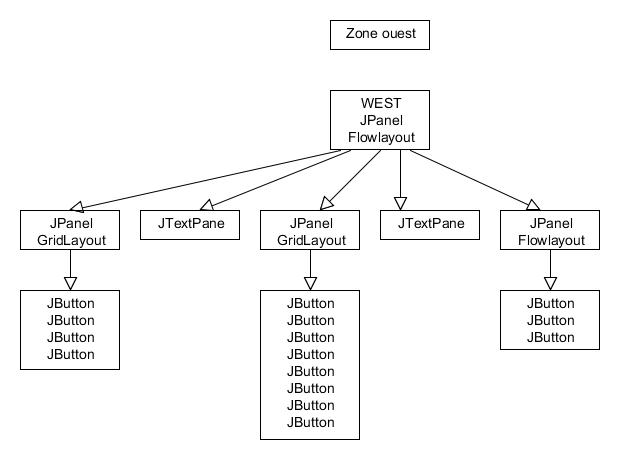
\includegraphics[scale = 0.7]{arbre_jframe_ouest.jpg}
	\caption{Hiérarchie des objets de la zone ouest de la fenêtre}
	\end{center}
\end{figure}
\newpage
Ensuite, l'organisation des éléments dans la fenêtre est la suivante :

\begin{figure}[!h]
\begin{center}
   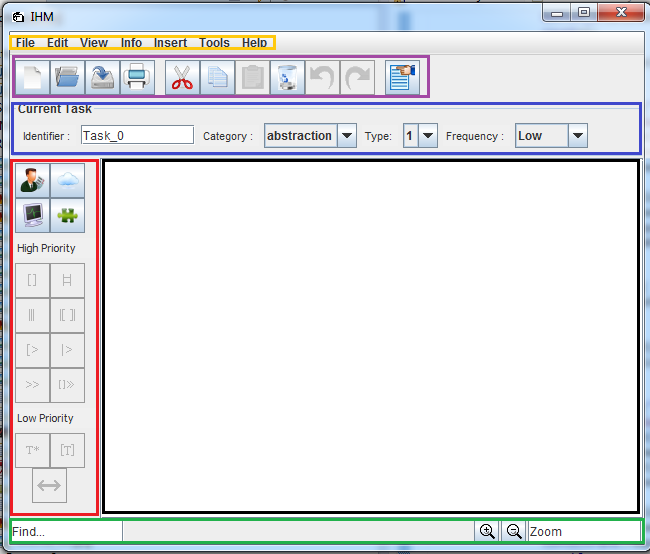
\includegraphics[scale = 0.9]{interface.png}
	\caption{Notre interface}
	\end{center}
\end{figure}
\newpage
\begin{itemize}
\item [*]La zone jaune représente les différents menus avec la grande majorité des options spécifiques, tel que la sauvegarde en jpg, l'accès à l'aide, etc... 
\item [*]La zone violette regroupe les différents outils de manipulation rapide de fichier. Ils sont triés par sous groupe en fonction de leur utilisation. 
\item [*]La zone suivante, en bleu, permet de voir en temps réel les informations du nœud sélectionné (le nœud courant), et de les modifier au besoin. 
\item [*]La zone noire représente la zone de travail où l'arbre s'affiche. 
\item [*]En rouge, il s'agit de la zone de travail sur les nœuds, pour leur création, ou les opérateurs d'association. 
\item [*]Enfin, la zone verte permet à l'utilisateur d'utiliser la recherche d'un nœud dans l'arbre, et la fonctionnalité zoom.
\end{itemize}

\newpage
\textcolor{Violet}{\section{Spécifications techniques}}

\textcolor{NavyBlue}{\subsection{Nos choix}}

En premier lieu, nous avons décidé d'enlever un certain nombre de boutons de la fenêtre. Pour commencer, nous avons jugé que la sauvegarde en temps que \emph{JPG} n'est pas de première nécessité et n'est pas souvent utiliser. De même, nous avons considéré qu'une personne utilisera plus souvent les options de copiage et de coupage par \emph{SubTree}, donc nous avons retiré de la barre la fonction \emph{Cut}. Toujours en suivant ce raisonnement, pour nous le \emph{check model structur} et \emph{insert mode} ne sont pas de première importance, comme les 4 boutons de travaux sur la hauteur des arbres. Nous estimons également que le zoom n'est pas agréable à utiliser, nous avons préféré prendre un système ou l'utilisateur aurait toujours le choix de la valeur de zoom, ou bien mettre un zoom par un pas prédéfini, et placer les options en bas à droite de l'écran de manière plus discrète. Nous avons définitivement enlevé les options de modification du texte.Dans notre façon de voir, ce sont des choses atteignable par clique droit / propriété ou en cliquant sur le bouton propriété d'un nœud. Pour les choix de conceptions , nous nous sommes principalement basés sur l'ihm du logiciel \emph{Word} et de notre utilisation de ce dernier. Ainsi nous n'utilisons ce logiciel que pour fournir, majoritairement des documents succins, où nous allons directement à l'essentiel. Par conséquent et à titre d'exemple, la modification de la police et de la taille de caractère passe au second plan et ne sera utilisée que pour le rendu final.\\


Nous avons par la suite supprimé \emph{l'overview}, qui pour nous ne présente aucun intérêt. Un utilisateur préfèrera selon nous se déplacer sur son espace de travail plutôt que de regarder dans un \emph{overview} trop petit pour fournir des informations pertinentes. Nous avons garder la zone de modification rapide d'un nœud, en apportant une modification. Nous avons créé une liste déroulante pour le type. En effet, ce champ attend toujours une valeur précise, plutôt que de la faire rentré par un utilisateur qui pourrait se tromper, nous fournissons la liste des types que l'utilisateur choisi. Nous avons également enlevé la plateforme, qui est disponible dans les paramètres complets accessible comme expliqué précédemment.\\



Pour le bandeau de gauche, nous l'avons rendu plus visible car celui-ci nous parait écrasé dans CTTE. Pour cela, nous avons décidé de faire deux colonnes de boutons. Nous les avons tous gardés, car nous estimons qu'ils sont tous important. Nous avons choisi en revanche de fournir des infobulles plus conséquentes, afin de mieux aider un utilisateur novice à comprendre les différentes fonctions.\\


Afin de rendre le logiciel plus ``jeune'', nous avons décidé de mettre de nouvelles icônes. En particulier, la sauvegarde est désormais un disque dur avec une flèche, les disquettes ayant disparues de nos espaces de travail. Nous avons ajouté une fonction de recherche, car dans les grands arbres, il peut être difficile de s'y retrouver. Pouvoir chercher un nœud en particulier nous parait important. Nous avons placé ce bouton de manière discrète en bas à gauche.\\


Afin de moins surcharger les menus, nous avons décidé de regrouper les différentes options de sauvegarde dans un même onglet, nommé \emph{Save as}. Nous avons ajouté un bandeau \emph{Help}, proposant un tutoriel, également proposé à la première ouverture du logiciel, et une section aide avec possibilité d'effectuer une recherche dedans.\\


Nous avons ré implémenté la totalité des options, ainsi que les raccourcis, en ajoutant les raccourcis MacOS avec la touche \emph{Command} (comme spécifié plus tard). Une demande de confirmation pour quitter le logiciel est demandé, afin de s'assurer que l'utilisateur ne quittera pas par erreur sans enregistrer son travail. De même, nous avons placé une taille de fenêtre minimal (inséré la valeur créée ici).

\textcolor{NavyBlue}{\subsection{Raccourcis clavier}}

Un large choix de raccourcis clavier ont été ajoutés sur le logiciels, fonctionnant sous Windows, Linux ou Mac OS X (Testé sur la version 10.6.8)

\begin{tabular}{| c | c | c |}
\hline
Fonction & Raccourcis avec CTRL & Raccourcis avec Command \\ \hline
Trouver & CTRL + F & Command + F \\ \hline
Arbre prioritaire & CTRL + T & Command + T \\ \hline
Copier & CTRL + C & Command + C \\ \hline
Coller  & CTRL + V & Command + V \\ \hline
Couper & CTRL + X & Command + X \\ \hline
Nouveau niveau & CTRL + L & Command + L \\ \hline
Fold / Unfold sous arbre & CTRL + H & Command + H \\ \hline
Unfold tout & CTRL + U & Command + U \\ \hline
Retour avant & CTRL + Z & Command + Z \\ \hline
Retour arrière & CTRL + Y & Command + Y \\ \hline
Description informelle à description formelle & CTRL + D & Command + D \\ \hline
Imprimer & CTRL + P & Command + P \\ \hline
Reachablelity analysis  & CTRL + A & Command + A \\ \hline
Ouvrir & CTRL + O & Command + O \\ \hline
Nouveau & CTRL + N & Command + N \\ \hline
Coller SubTree & CTRL + SHIFT + V & Command + SHIFT + V \\ \hline
Copier SubTree & CTRL + SHIFT + C & Command + SHIFT + C \\ \hline
Ouvrir CTT en tant que XML  & CTRL + SHIFT + O & Command + SHIFT + O \\ \hline
Enregistrer en tant que... & CTRL + SHIFT + S & Command + SHIFT + S \\ \hline
Imprimer en plusieurs pages & CTRL + SHIFT + P & Command + SHIFT + P \\ \hline
Model Filter & CTRL + SHIFT + F & Command + SHIFT + F \\ \hline
Supprimer & Supprimer & / \\ \hline
Inserer sous arbre par fichier & Insert & / \\ \hline
Vérification de la structure du modèle & F7 & / \\ \hline
Start task model simulator & F4 & / \\ \hline
\end{tabular}

\textcolor{Violet}{\section{Les critères de Scapin et Bastien et notre interface}}

\textcolor{NavyBlue}{\subsection{Incitation}}

Afin de mieux aider l'utilisateur, nous avons grisé des boutons pour l'utilisation des différentes fonctionnalités qui ne sont pas utilisables à un instant T (comme par exemple la possibilité de copier si il n'y a rien à copier, ou la manipulation sur les arbres si il n'y en a pas). 

\textcolor{NavyBlue}{\subsection{Groupement / Distinction entre items}}

Nous avons décidé de conserver une logique quand au regroupement des boutons pour notre interface, en fonction de leur utilité. les opérations générales sont dans un bandeau en haut du document, les opérations sur les arbres sont également regroupées sur la gauches dans un autre bandeau. Nous avons également fait attention à bien séparer les groupements de boutons, pour plus de lisibilité. Des options, comme les différentes possibilités de sauvegarde, sont regroupées dans des sous menus de la barre des menus.

\newpage
\textcolor{NavyBlue}{\subsection{Feedback immédiat}}

Pour aider l'utilisateur, une fonctionnalité sélectionnée apparait grâce à un marqueur sur le bouton qui est utilisé. De même, lorsque l'utilisateur passe en survolant un bouton avec sa souris, celui-ci devient légèrement plus foncé, pour lui indiquer où il se trouve. De plus, grâce au bouton sauvegarder qui se grise si le document n'a pas subit de modification, l'utilisateur sait exactement où il en est dans son travail à n'importe quel moment. Enfin, notre zone d'édition simplifiée pour un nœud se met à jour à chaque création de nœud ou édition de celui-ci, permettant à l'utilisateur d'avoir une vue sur ces modifications (par exemple, si il change le nom dans le champ correspondant et appuie sur entré, le nom de la tâche se met à jour).

\textcolor{NavyBlue}{\subsection{Lisibilité}}

En premier lieu, il est important de constater que notre interface contient bien moins de boutons que l'interface originelle de CTTE. Nous avons décidé de garder le minimum d'option avec le maximum d'efficacité. Nous avons donc enlevé la plupart des options que nous ne jugions pas adéquates. Nous avons également décidé de regrouper des options dans le menu \emph{file}, notamment pour la sauvegarde afin de ne pas surcharger l'interface d'options au risque d'effrayer l'utilisateur.

\textcolor{NavyBlue}{\subsection{Densité informationnelle}}

Pour notre prototype, comme expliqué précédemment, nous avons décidé d'enlever la plupart des boutons et de regrouper des options dans les menus, afin de rendre l'interface plus agréable à l'utilisateur et moins chargée.

\textcolor{NavyBlue}{\subsection{Actions explicites - Contrôle utilisateur}}

L'utilisateur possède le plein contrôle des actions de notre prototype, ajouter un nœud, le modifier, le supprimer, effectuer une opération sur un arbre, etc... L'utilisateur peut également annuler ou refaire une action qu'il aurait annulé à l'aide des boutons \emph{undo} et \emph{redo}.

\textcolor{NavyBlue}{\subsection{Prise en compte de l'expérience utilisateur}}

A la différence de CTTE, nous avons décidé d'accorder une place plus grande sur la prise en compte de l'expérience utilisateur. Pour commencer, nous avons décidé de proposer un tutoriel à la première ouverture du logiciel, pour aider les novices à découvrir le logiciel. De plus, nous avons décidé d'ajouter un menu d'aide pour aider ces utilisateurs à prendre en main le logiciel. Nous avons également rajouté des informations sur les infobulles des boutons d'opérations sur les arbres.\\


Pour les utilisateurs experts, nous avons implémenté tous les raccourcis de CTTE, autant les combinaisons par la touche \emph{CTRL} (avec ``x'' pour couper, ``s'' pour sauvegarder) que \emph{ALT} (avec ``f'' pour ouvrir le menu file par exemple) ou \emph{Command}. Ainsi, ils peuvent effectuer les opérations qu'ils connaissent de manière plus rapide. 
\textcolor{NavyBlue}{\subsection{Protection contre les erreurs}}

Pour protéger l'utilisateur des erreurs simples, nous avons décidé de griser les boutons lorsqu'ils ne sont pas utilisables. Nous avons également modifié le type du champ \emph{Current task} qui posait problème. Il s'agit d'une liste déroulante évitant ainsi que l'utilisateur ne se trompe dans la saisie de la donnée. Enfin, notre logiciel effectue un rappel à l'utilisateur quand à la sauvegarde, pour éviter une perte d'un document à l'insu de l'utilisateur.

\textcolor{NavyBlue}{\subsection{Signifiance des codes et dénomination}}

Dans notre prototype, nous avons gardé des infobulles explicites en rapport avec la fonctionnalité des boutons, et nous avons au besoin rajouté des informations complémentaires pour la compréhension de certaines. Nous avons également mis des images donnant un ``coup de jeune'' à l'application, plus grandes, par exemple la sauvegarde avec un disque dur et non une disquette.

\textcolor{NavyBlue}{\subsection{Compatibilité}}

Pour notre interface, une taille minimum est obligatoire (650 x 550). De plus, nous avons décidé d'adapter le style de la fenêtre en fonction du système d'exploitation. Ainsi, sur un Windows 7 par exemple, les différentes pop-up qu'affichera le prototype seront dans le thème Aero si l'utilisateur utilise le thème Aero, ou dans le thème XP si il utilise un thème de type Windows XP.

\textcolor{Violet}{\section{Fonctionnalités non disponibles}}

Notre prototype n'est qu'une interface, et la création d'un arbre n'est donc pas réalisable. La plupart des options ne font qu'ouvrir des pop-up. La sauvegarde et l'ouverture de fichier ne fonctionnent également pas.
\end{document}